\documentclass{article}
\usepackage[utf8]{inputenc}
\usepackage[portuguese]{babel}
\usepackage[top=1in, bottom=1in, left=1in, right=1in]{geometry}
\usepackage{graphicx}
\usepackage{indentfirst}
% \usepackage{verbatim}

\setlength{\parindent}{20pt}

\title{Inteligência Artificial - Trabalho 1\\Jogo dos Palitos}
\author{Caio Pereira Oliveira, Salomão Rodrigues Jacinto e William Kraemer Aliaga}
\date{Abril de 2017}


\begin{document}

\maketitle

\section{Regras}

\begin{itemize}

\item Usam-se palitos ou qualquer outro material que possa ficar dentro da palma da mão.
\item Pode ser jogado de 2 a várias pessoas. Cada pessoa terá 3 palitos e terá de escolher uma quantidade a colocar na mão sem que os adversários saibam.
\item Depois todos deixam a mão fechada sobre a mesa, então cada jogador apostará o valor da soma de todos os palitos na mão de cada um.
\item Quem acerta o total retira um de seus palitos disponíveis e se torna o primeiro a apostar.
\item Ganha aquele que ficar sem nenhum palito, após ter acertado repetidas vezes seu palpite.

\end{itemize}

\section{Detalhes de Implementação}

Para implementação deste trabalho foi utilizada a linguagem Python por suportar multiparadigmas e ter algumas facilidades como \textit{list comprehensions}.

Foram implementados três tipos de jogadores: uma interface para um jogador humano participar do jogo, a inteligência artificial e um jogador que sempre escolhe números aleatórios.

Existem também duas classes que gerenciam o jogo: \emph{Match} e \emph{Game}, \emph{Match} cuida de uma partida que começa com cada jogador escolhendo quantos palitos terá em sua mão e termina quando todos os jogadores fizeram um palpite ou um jogador acertar a soma do número de palitos. Já \emph{Game} gerencia as rodadas removendo os palitos dos vencedores e verificando o fim do jogo.


\section{Algoritmos}

Dentro da probabilidade e estatística é comumente utilizado para modelar fenômenos naturais o que é chamado de distribuição normal, essa distribuição é parametrizada baseada na média e na variância, ou desvio padrão, que indicam a regularidade de um conjunto de dados. A imagem abaixo descreve a soma de 10 números aleatórios realizado 10 mil vezes e transformado em um gráfico de barras. Traçando um gráfico através dessa imagem mostra que ela se assemelha a uma distribuição normal centrada com um desvio padrão um pouco maior que a distribuição normal padrão.

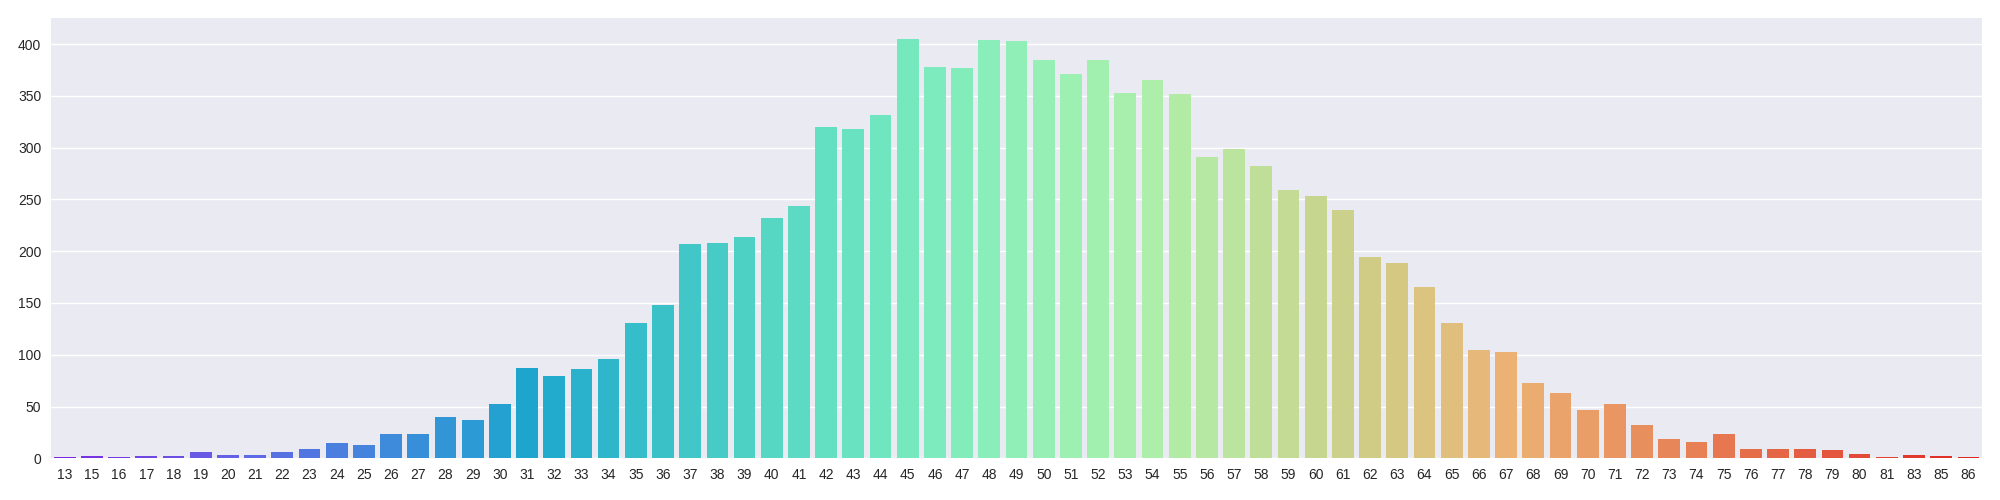
\includegraphics[width=\textwidth]{soma_de_randoms}

Como o jogo no qual está se construindo uma inteligência artificial se baseia na soma de números aleatórios a heurística utilizada foi uma forma de média ponderada para que a inteligência através do palpite e do número máximo que um jogador poderia ter jogado tente adivinhar quantos palitos ele está na mão, e fazendo isso com todo os jogadores anteriores a ele consegue eliminar os extremos do palpite e tentar convergir para o que serão os melhores palpites com as informações que ele possuí. Foram utilizadas duas listas para conter os dados necessários para IA.

\section{Testes}

Para testar a eficácia da inteligência criada foi criada uma funcionalidade de simulação, desta forma é possível executar milhares de jogos da inteligência artificial contra jogadores que sempre escolhem números aleatórios.

Foram feitas as seguintes simulações, todas com 100 mil jogos:

(Os números ao lado de cada jogador representam o número de jogos que ele ganhou)

\begin{itemize}

\item Um jogador inteligente contra um jogador aleatório:

\begin{verbatim}
AI_0: 56371
Random_0: 43629
\end{verbatim}


\item Dois jogadores inteligentes contra um jogador aleatório:

\begin{verbatim}
AI_1: 37365
AI_0: 37076
Random_0: 25559
\end{verbatim}


\item Um jogador inteligente contra dois jogadores aleatórios:

\begin{verbatim}
AI_0: 43189
Random_1: 28607
Random_0: 28204
\end{verbatim}


\item Dois jogadores inteligentes contra dois jogadores aleatórios:

\begin{verbatim}
AI_0: 32404
AI_1: 32164
Random_1: 17847
Random_0: 17585
\end{verbatim}

\end{itemize}


\section{Opções de execução do programa}

\begin{verbatim}
> python3 palitos.py [argumentos]
\end{verbatim}

Argumentos disponíveis:

\begin{verbatim}
--help                exibe a mensagem de ajuda e termina
-a N, --ai N          número de jogadores inteligentes (default: 0)
-r N, --random N      número de jogadores aleatórios (default: 0)
-p P, --picks P       número inicial de palitos (default: 3)
-h NAME [NAME ...], --human NAME [NAME ...]
                    adiciona jogadores humanos
-v, --verbose         aumenta o nível de verbose
-s N, --simulate N    simula N jogos. não pode ser utilizado junto com "-h"

\end{verbatim}


\subsection{Exemplos de uso:}

\begin{itemize}

\item Executa um jogo com um jogador inteligente e um jogador aleatório.
\begin{verbatim}
> python3 palitos.py -a 1 -r 1
\end{verbatim}


\item Executa um jogo com um jogador inteligente, um jogador aleatório e um jogador humano chamado "Human\_1".
\begin{verbatim}
> python3 palitos.py -a 1 -r 1 -h Human_1
\end{verbatim}

\item Executa um jogo com um jogador inteligente, um jogador aleatório e dois jogadores humanos chamados "Human\_1" e Human\_2.
\begin{verbatim}
> python3 palitos.py -a 1 -r 1 -h Human_1 Human_2
\end{verbatim}

\item Executa um jogo com dois jogadores inteligentes e um jogador aleatório, cada jogador iniciando com 5 palitos.
\begin{verbatim}
> python3 palitos.py -a 2 -r 1 -p 5
\end{verbatim}

\item Simula 10 mil jogos com um jogador inteligente e um jogador aleatório.
\begin{verbatim}
> python3 palitos.py -a 1 -r 1 -s 10000
\end{verbatim}

\end{itemize}

\end{document}
